\documentclass[sigconf,natbib=true,anonymous]{acmart}
%% RecSys 2026 — 主会长文（8 页正文 + 参考文献不限）
%% 使用 ACM sigconf 版式（双栏），双盲审稿。
%% 终稿：去掉 anonymous 并填写作者信息。
%% 编译：建议使用 XeLaTeX 或 LuaLaTeX（与 ctex 配合）。

%% Remove ACM-specific elements for cleaner review copy
\settopmatter{printacmref=false}
\renewcommand\footnotetextcopyrightpermission[1]{}
\setcopyright{none}
\acmConference[RecSys'26]{Proceedings of the 20th ACM Conference on Recommender Systems}{September 2026}{TBD}
\acmYear{2026}
\acmDOI{}
\acmISBN{}

\usepackage{booktabs}
\usepackage{multirow}
\usepackage{amsmath,amssymb}
\usepackage{algorithm}
\usepackage{algpseudocode}
\usepackage{graphicx}
\usepackage{subcaption}
\usepackage{siunitx}
\usepackage{xspace}
\usepackage{enumitem}
\usepackage{microtype}
\setlength{\emergencystretch}{3em}
\usepackage{ifthen}
\usepackage{balance}
\usepackage{hyperref}
\usepackage{ctex}

\newcommand{\model}{\textsc{MV-Align}\xspace}
\newcommand{\base}{\textsc{SASRec}\xspace}
\newcommand{\tfidf}{\textsc{TF-IDF}\xspace}
\newcommand{\llm}{\textsc{LLM}\xspace}
\newcommand{\InfoNCE}{InfoNCE\xspace}

\usepackage{pifont}
\newcommand*\circled[1]{\ding{\numexpr171+#1\relax}}

\begin{document}

\title{MV-Align：面向序列推荐的多视角文本对齐与显式特征交叉}

\begin{abstract}
将文本特征融入序列推荐模型可显著提升泛化能力，尤其对冷启动物品；然而既有方法往往依赖单一文本表示，并仅通过共享注意力层与 ID 嵌入隐式融合。
我们认为该设计错失两点机会：(i)~由多样化提示驱动的多视角 \llm 表示能捕捉互补的物品语义，而单一嵌入难以涵盖；(ii)~ID 与文本信号之间的显式特征交叉——在 CTR 预测中已成熟，但在序列推荐中尚少探索——可提升排序质量。
%
我们提出 \model，在 \base 骨干之上引入三项协同设计：融合前对各视角 \llm 嵌入做\textbf{逐视角白化}以去相关；通过 DCN-V2 实现\textbf{显式的 ID$\times$Text 交叉交互}；以及带冷启动重加权的\textbf{多视角对比对齐}。
在 Amazon Beauty 与 Toys\&Games 上进行全量排序评估的对照消融中，我们实证刻画了全量排序下的\textbf{HR--排序权衡}：启用交叉网络以召回（HR）为代价提升排序精度（MRR/NDCG），关闭则相反——该发现直接对应候选生成与最终重排之间的部署取舍。
%
\model 取得 HR@10 为 \textbf{5.79}\% 与 \textbf{6.61}\%（相对仅 ID 为 +6.8\% 与 +11.7\%）；在嵌入带宽相同条件下，多视角提示在 Beauty 上将冷启动 HR\_new 与仅 ID 的差距缩小至 1.76\% 对 1.88\%，在 Toys 上则超过仅 ID（2.04\% 对 1.92\%），并在两个数据集上取得最优冷启动排序质量（NDCG\_new 与 MRR\_new）。
代码与配置见 \texttt{\url{https://anonymous.4open.science/r/recbole-multiview-D83A}}。
\end{abstract}

\keywords{序列推荐, 文本增强推荐, 多视角表示, 特征交叉, 对比对齐, 冷启动}

\maketitle

\section{引言}

现代序列推荐模型如 \base~\cite{kang2018sasrec} 为建模用户行为序列提供了强骨干，但现实目录中冷启动与长尾物品占主导，协同信号稀疏。物品文本（标题、描述、评论）可提供语义线索以改善泛化，但也带来工程张力：轻量特征（如 \tfidf）成本低且往往很强，而 \llm 嵌入更丰富，但在抽取、存储与在线服务上昂贵得多。

自然的问题是：多视角 \llm 特征是否值得额外复杂度。我们通过报告可训练参数量与前向 FLOPs（表~\ref{tab:params}）并在 \S\ref{sec:complexity} 中分析离线编码成本来量化这一点。

两项实践观察驱动本工作。第一，一旦较强的 \tfidf 基线就位（例如 Beauty 全量排序下 HR@10 +2.6\%、NDCG@10 +25.9\%），再叠加 \llm 特征的边际收益可能较小且因域而异，难以判断多视角提示是否值得额外离线编码与适度增加的可训练开销（\S\ref{sec:experiments}）。第二，工业界模型选型常依赖快速采样评估（均匀 100 负例），但采样指标可能与全量排序不一致甚至错排模型~\cite{krichene2020sampledmetrics}；当改进集中在冷启动/长尾层时，这种错配尤其有害。

\model 以简单的「准备--交互--对齐」流程应对上述矛盾（图~\ref{fig:framework}）：

\textbf{(1) 准备}（表示层）：我们对每个文本视角独立归一化与白化，以应对三类失效模式——视角间尺度不匹配、视角间相关、以及跨视角冗余。白化使多视角通道去相关，使后续交互更易学习。

\textbf{(2) 交互}（融合层）：我们使用显式交叉网络（DCN-V2）学习高阶 ID$\times$text 特征交叉。虽然 Transformer 自注意力建模序列级物品--物品依赖，但并不显式刻画 ID 嵌入与文本嵌入之间的特征级交互；DCN-V2 通过由学习到的权重矩阵门控的元素乘积填补这一空白。

\textbf{(3) 对齐}（目标层）：我们通过 InfoNCE 对比损失将各文本视角对齐到协同 ID 嵌入空间。对齐方向为（文本视角 $\to$ ID 空间）；正样本为（物品的文本视角，物品的 ID 嵌入）；负样本为 batch 内物品。冷启动重加权避免高频物品主导对齐信号，使低流行度物品获得足够梯度更新。

我们的贡献有三点。
\begin{itemize}[leftmargin=*,itemsep=1pt]
  \item \textbf{系统性的方法设计。} 我们提出 \model，将显式交叉网络（DCN-V2）与多视角 \llm 文本特征结合用于序列推荐。「准备--交互--对齐」设计联合利用逐视角白化、显式 ID$\times$Text 交叉，以及带冷启动重加权的对比对齐——据我们所知，该组合在此设定下尚未被探索。
  \item \textbf{新的实证发现。} 在两个 Amazon 域上进行全量排序评估并结合流行度分层分析的对照消融中，我们揭示此前未报道的\textbf{HR--排序权衡}：交叉网络以召回（HR）为代价提升排序质量（MRR/NDCG），为从业者在候选生成与最终重排配置之间选择提供可操作的指导。
  \item \textbf{实践设计洞见。} 我们表明单独的轻量 \tfidf 已是出人意料的强基线；在相同嵌入带宽（$4{\times}64$ 维 对 $1{\times}256$ 维）下，多视角提示稳定优于单视角，冷启动物品上增益最大。
\end{itemize}
围绕四个研究问题组织本文：
\textbf{RQ1}~逐视角白化是否改善文本特征质量？
\textbf{RQ2}~SE 式通道门控是否有帮助？
\textbf{RQ3}~在相同嵌入带宽下，多视角是否优于单视角？
\textbf{RQ4}~显式交叉与对比对齐各自的贡献是什么？
余下结构：相关工作、\model 方法、全量排序结果与消融、以及分析与总结。

\section{相关工作}
\paragraph{序列推荐。}
基于 Transformer 的序列模型如 \base~\cite{kang2018sasrec} 与 BERT4Rec~\cite{sun2019bert4rec}（采用双向掩码预测）是刻画用户行为模式的强骨干。
GRU4Rec~\cite{hidasi2016gru4rec} 开创了基于 RNN 的会话建模，而 SASRec 将自注意力用于带因果掩码的下一物品预测。近期高效变体包括采用低秩注意力分解以降低复杂度的 LightSANs~\cite{fan2021lightsans}。

\paragraph{文本增强推荐。}
\begin{sloppypar}
物品文本特征（词袋、神经编码器或 \llm 嵌入）在协同过滤之外提供互补信号。早期工作使用 TF-IDF 与 Item2Vec~\cite{barkan2016item2vec} 表示物品；
CDL~\cite{wang2015cdl} 通过堆叠去噪自编码器联合建模文本。近期方法利用预训练语言模型：UniSRec~\cite{hou2022unisrec} 将 BERT 编码的物品文本作为通用可迁移表示，VQ-Rec~\cite{hou2023vqrec} 通过向量量化桥接语言与协同语义。大语言模型进一步拓展该方向：
P5~\cite{geng2022p5} 以文本到文本范式统一推荐，TALLRec~\cite{bao2023tallrec} 通过指令微调对齐 LLM 与推荐。
然而，这些方法通常以单一提示或表示编码物品文本。
我们探索通过多样化提示视角（身份、功能、受众、类别）得到的\textbf{多视角} \llm 嵌入，配合显式融合与对齐，并展示相对更简单方案何时值得引入该额外复杂度。
\end{sloppypar}

\paragraph{特征交互与交叉网络。}
Deep \& Cross Network (DCN)~\cite{wang2017dcn} 及其后继 DCN-V2~\cite{wang2021dcnv2} 显式建模特征交叉，补充 DNN 学到的隐式交互。
Squeeze-and-Excitation (SENet)~\cite{hu2018senet} 引入通道注意力以自适应重标定特征；FiBiNET~\cite{huang2019fibinet} 将 SENet 适配到 CTR 预测并加入双线性特征交互。
推荐中交叉网络在 CTR 上已证明有效；我们将其适配于序列设定下的 ID--文本融合，并用 SE 式模块对 \llm 特征做逐视角通道门控。

\paragraph{推荐中的多视角学习。}
多视角学习利用不同特征源或模态的互补信息。受 CLIP~\cite{radford2021clip} 通过对比学习对齐视觉与文本表示的启发，我们设计多视角提示以从语言模型中引出多样语义。
推荐中已有面向会话场景的多视角图神经方法~\cite{huang2025mvcgnn_session}。我们将多视角学习应用于 \llm 文本嵌入，采用不同提示视角（身份、功能、受众、类别）并在融合前通过白化使视角表示去相关。

\paragraph{推荐中的对比学习。}
\InfoNCE~\cite{oord2018cpc} 等对比目标广泛用于自监督表示学习。推荐中对比方法在用户/物品表示跨视角对齐~\cite{wu2021cl4rec}。
我们将其扩展到带冷启动重加权的多视角文本到 ID 对齐。

\paragraph{评估协议。}
采样评估可能误导模型选择~\cite{krichene2020sampledmetrics}；全量排序评估更可靠但计算昂贵。我们采用全量排序并结合分层分析以理解不同流行度层上的行为。

\section{方法}
图~\ref{fig:framework} 展示了 \model 的整体架构。框架包含三个关键部分：
(1)~\textbf{归一化与白化}，每个文本视角经逐视角归一化以缓解各向异性；
(2)~\textbf{交叉网络}，通过 DCN-V2 捕获显式 ID$\times$Text 交互；
(3)~\textbf{多视角对齐}，使用带冷启动重加权的 InfoNCE 损失将文本视角与 ID 嵌入对齐。
下文分别详述。

\subsection{骨干：融合文本的 SASRec}
设用户交互序列为 $s_u = [i_1,\dots,i_n]$，最大长度为 $L$。\base 通过 Transformer 将 $s_u$ 编码为序列表示 $\mathbf{h}_u \in \mathbb{R}^d$。每个物品 $i$ 有 ID 嵌入 $\mathbf{e}_i \in \mathbb{R}^d$。我们为物品增加文本特征并融合为用于打分的\textbf{融合物品嵌入} $\tilde{\mathbf{e}}_i$。

\subsection{多视角文本表示}\label{sec:whiten}
假设轻量 \tfidf 嵌入 $\mathbf{t}_i^{(0)} \in \mathbb{R}^{d_t}$ 为基视角，并有 $V$ 个 \llm 提示视角 $\{\mathbf{t}_i^{(v)} \in \mathbb{R}^{d_l}\}_{v=1}^V$（如身份/功能/受众/类别），其中 $d_t$、$d_l$ 分别为 \tfidf 与原始 \llm 嵌入维度。

\paragraph{逐视角白化。}
多视角 \llm 嵌入存在三类失效模式：
\textbf{(i) 尺度不匹配}——不同视角幅度分布差异大，导致部分视角主导融合；\textbf{(ii) 视角相关}——引出相似语义的提示产生相关特征，冗余编码同一信息；\textbf{(iii) 跨视角冗余}——不去相关时，交叉网络跨视角学到冗余交互而非互补交叉。

为此，我们先将每个 \llm 视角从 $d_l$ 经截断 SVD 降至 $d_v$ 维，再对每个视角独立应用 ZCA 白化~\cite{kessy2018zca}，使多视角通道去相关并利于后续交互学习。
给定视角 $v$ 上全体物品的降维嵌入矩阵 $\mathbf{X}^{(v)} \in \mathbb{R}^{|I| \times d_v}$，计算：
\begin{align}
  \mathbf{X}_c^{(v)} &= \mathbf{X}^{(v)} - \boldsymbol{\mu}^{(v)}, \\
  \boldsymbol{\Sigma}^{(v)} &= \frac{1}{|I|}(\mathbf{X}_c^{(v)})^\top \mathbf{X}_c^{(v)}, \\
  \mathbf{X}_w^{(v)} &= \mathbf{X}_c^{(v)} (\boldsymbol{\Sigma}^{(v)} + \epsilon \mathbf{I})^{-1/2},
\end{align}
其中 $\boldsymbol{\mu}^{(v)}$ 为均值嵌入，$\boldsymbol{\Sigma}^{(v)}$ 为协方差，$\epsilon$ 为小常数以保证数值稳定。白化统计在训练集上离线计算并在训练/推理时固定。每个视角使用独立白化参数（逐视角白化），比跨视角共享白化更能保留视角特有语义。

\paragraph{SE 式通道门控。}
我们使用 SE 式通道门控进行自适应特征重标定，灵感来自 SENet~\cite{hu2018senet} 的通道注意力。原始 SENet 先 squeeze（全局池化）再 excitation，而我们对每个投影嵌入直接应用基于 MLP 的门控，更适合逐物品表示（不在物品间池化）。每个白化视角投影到骨干维度 $d$ 并精炼为：
\begin{align}
  \mathbf{z}_i^{(v)} &= \mathbf{W}_v \mathbf{t}_{w,i}^{(v)} \in \mathbb{R}^d,\\
  \mathbf{r}_i^{(v)} &= \mathbf{z}_i^{(v)} \odot \sigma(\mathrm{MLP}_v(\mathbf{z}_i^{(v)})),
\end{align}
其中 $\mathbf{W}_v \in \mathbb{R}^{d \times d_v}$ 为投影矩阵，$\mathbf{t}_{w,i}^{(v)} \in \mathbb{R}^{d_v}$ 为物品 $i$ 在视角 $v$ 的白化嵌入，$\mathrm{MLP}_v: \mathbb{R}^d \to \mathbb{R}^d$ 为降维比 $r$ 的两层网络。

\paragraph{逐视角 $\ell_2$ 归一化。}
SE 门控后，我们对每个视角独立做 $\ell_2$ 归一化。目的有二：(i) 保证各视角以可比尺度参与融合，避免大幅度视角主导；(ii) 通过良好条件的输入稳定后续交叉网络学习：
\begin{equation}
  \hat{\mathbf{r}}_i^{(v)} = \frac{\mathbf{r}_i^{(v)}}{\lVert \mathbf{r}_i^{(v)} \rVert_2 + \epsilon}.
\end{equation}
与白化结合，逐视角归一化在保留各视角语义的同时缓解尺度不匹配：白化去相关各视角内部维度，$\ell_2$ 归一化使跨视角贡献幅度可比。

\paragraph{视角门控与融合。}
我们为每个视角学习标量门 $g_v=\sigma(\theta_v)\in(0,1)$，且\textbf{不}强制跨视角归一化（各视角独立贡献 $0$--$1$）。所有视角（及可选的 \tfidf 基）拼接后投影回 $\mathbb{R}^d$：
\begin{equation}
  \mathbf{t}_i = \mathbf{P}\Big[\mathbf{t}_i^{(0)};\; g_1\hat{\mathbf{r}}_i^{(1)};\; \dots;\; g_V\hat{\mathbf{r}}_i^{(V)}\Big] \in \mathbb{R}^d,
\end{equation}
其中 $\mathbf{P} \in \mathbb{R}^{d \times (d_t + Vd)}$ 为融合投影矩阵。

\subsection{显式交叉融合}\label{sec:cross}
除依赖自注意力捕获协同与文本的高阶交互外，我们引入基于 DCN-V2~\cite{wang2021dcnv2} 的\textbf{显式交叉}模块。\base 中的自注意力建模序列级物品--物品依赖，但不显式建模 ID 嵌入与文本嵌入之间的特征级交叉；DCN-V2 通过学习到的权重矩阵门控的元素乘积学习高阶 ID$\times$text 交互。

设拼接特征 $\mathbf{x}_i=[\mathbf{e}_i;\alpha_i \mathbf{t}_i] \in \mathbb{R}^{2d}$，其中 $\mathbf{e}_i$ 为 ID 嵌入，$\mathbf{t}_i$ 为融合文本表示，交叉层更新为：
\begin{equation}
  \mathbf{x}^{(l+1)} = \mathbf{x}^{(l)} + \mathbf{x}^{(0)} \odot (\mathbf{W}_l\mathbf{x}^{(l)} + \mathbf{b}_l),
\end{equation}
其中 $\mathbf{W}_l \in \mathbb{R}^{2d \times 2d}$ 为满秩权重，$\mathbf{b}_l$ 为偏置；$\odot$ 为逐元素乘积。我们使用 DCN-V2 的满秩变体（非 mix），而非低秩或混合专家变体。
交叉输出 $\mathbf{x}^{(C)} \in \mathbb{R}^{2d}$ 与浅层 MLP 经预测层组合得到融合嵌入 $\tilde{\mathbf{e}}_i \in \mathbb{R}^d$。
标量 $\alpha_i \in (0,1)$ 包含全局文本门与可选的逐物品门控，并按温度缩放以稳定融合。

\subsection{多视角对比对齐}\label{sec:align}
我们使用 \InfoNCE~\cite{oord2018cpc} 将各文本视角对齐到 ID 嵌入空间。对齐目标为：\textbf{文本视角 $\to$ ID 空间}；正样本为（物品的文本视角，物品的 ID 嵌入）；负样本为 batch 内物品。这使文本表示携带协同信号，在冷启动场景可作为 ID 嵌入的即插即用替代。

对 batch 大小 $B$，定义余弦相似度矩阵 $\mathbf{S} \in \mathbb{R}^{B \times B}$，元素为 ID 嵌入 $\mathbf{e}_i$ 与文本视角嵌入 $\hat{\mathbf{r}}_{j}^{(v)}$ 之间的 $\mathrm{cos}(\cdot,\cdot)$，温度为 $\tau$。逐视角对齐损失为：
\begin{equation}
  \mathcal{L}_{\text{align}}^{(v)} =
  \frac{1}{B}\sum_{i=1}^{B}
  -\log \frac{\exp(\mathbf{S}_{ii}/\tau)}{\sum_{j=1}^{B}\exp(\mathbf{S}_{ij}/\tau)}.
\end{equation}
学习视角权重 $\pi_v=\mathrm{softmax}(\boldsymbol{\phi})_v$ 并组合：
\begin{equation}
  \mathcal{L}_{\text{mv-align}} = \sum_{v=1}^{V}\pi_v \mathcal{L}_{\text{align,w}}^{(v)}.
\end{equation}

我们通过两个阶段起作用的两种互补机制增强冷启动物品表现：

\paragraph{训练期冷启动重加权。}
为避免对齐被高频物品主导，我们按物品流行度 $\mathrm{pop}(i)$（交互次数）在训练时重加权样本：
\begin{equation}
  w_i = 1 + \beta\cdot \max\Big(0, \frac{P_0-\mathrm{pop}(i)}{P_0}\Big),
  \label{eq:cold_reweight}
\end{equation}
其中 $\beta>0$ 控制基于流行的重加权强度，$P_0$ 为冷启动阈值（$\mathrm{pop}(i) < P_0$ 的物品获得更大权重）。加权对齐损失为：
\begin{equation}
  \mathcal{L}_{\text{align,w}}^{(v)} =
  \frac{1}{\sum_i w_i}\sum_{i=1}^{B} w_i \cdot
  \left[-\log \frac{\exp(\mathbf{S}_{ii}/\tau)}{\sum_{j=1}^{B}\exp(\mathbf{S}_{ij}/\tau)}\right],
\end{equation}
其中 $w_i$ 仅重加权锚点（正）样本，确保冷启动物品在对齐训练中获得足够梯度。

\paragraph{推理期冷启动增强。}
为补充训练期重加权，我们在推理时自适应调整文本权重。对流行度为 $\mathrm{pop}(i)$ 的物品 $i$，计算动态增强因子：
\begin{equation}
  \gamma_i = 1 + \beta_{\text{infer}} \cdot \max\Big(0, 
  \frac{P_0-\mathrm{pop}(i)}{P_0}\Big),
  \label{eq:infer_boost}
\end{equation}
其中 $\beta_{\text{infer}}$ 为推理增强系数。融合层中有效文本权重变为 $\alpha_i' = \alpha_i \cdot \gamma_i$，在不改模型参数的情况下动态增大冷启动物品对文本的依赖。
该解耦允许部署时调节而无需重训：较小的 $\beta_{\text{infer}}$ 使整体指标更均衡，较大值更强调冷启动。
我们在验证集上联合调节 $\beta_{\text{infer}}$ 与 $(\lambda,\tau)$ 及训练重加权系数 $\beta$（式~\eqref{eq:cold_reweight}）；\S\ref{sec:analysis} 中的默认值（$\beta{=}3.0$，$\beta_{\text{infer}}{=}0.6$）体现了该权衡。

两种机制共同保证冷启动物品在训练期获得更强学习信号（重加权对齐），在推理期获得合适强调（动态增强），从而在不过度损害高频物品的前提下实现有效冷启动推荐。

\begin{figure}[t]
\centering
\IfFileExists{figures/framework.pdf}{%
  
\includegraphics[width=\linewidth]{figures/framework.pdf}%
}{%
  \fbox{\parbox[c][0.22\textheight][c]{0.95\linewidth}{\centering
  \textbf{框架图占位。}\\
  请将 `framework.pdf` 置于 `paper_sigir/figures/`。}}%
}
\caption{\model 概览。
\circled{1}~\textbf{准备}：逐视角归一化与白化（\S\ref{sec:whiten}）；
\circled{2}~\textbf{交互}：通过 DCN-V2 的显式 ID$\times$Text 交叉（\S\ref{sec:cross}）；
\circled{3}~\textbf{对齐}：带冷启动重加权的多视角对比对齐（\S\ref{sec:align}）。}
\label{fig:framework}
\end{figure}

\subsection{训练目标}
我们优化：
\begin{equation}
  \mathcal{L} = \mathcal{L}_{\text{rec}} + \lambda \cdot \mathcal{L}_{\text{mv-align}},
\end{equation}
其中 $\mathcal{L}_{\text{rec}}$ 为标准序列推荐损失（带采样负例的交叉熵），$\lambda$ 为对齐权重。负采样仅用于训练效率；所有评估指标在全物品集上全量排序计算。

\subsection{模型复杂度}\label{sec:complexity}
\textbf{离线。} \tfidf 与 \llm 物品嵌入预先计算一次并存为静态缓冲；SVD 降维与 ZCA 白化在训练集上离线完成。
每个 \llm 视角对每个物品需单独一次编码器前向，故离线编码成本大致随视角数增长（例如四提示视角对单视角）；这是一次性（或周期性刷新）成本，摊销到训练与服务，不增加单次请求延迟。
\textbf{在线。} 在线路径增加逐视角投影、一层 DCN-V2 交叉（$2d{\times}2d$）与融合 MLP。
表~\ref{tab:params} 报告 Amazon Beauty 上的可训练参数与框架估计的单次前向 FLOPs：文本融合与多视角头增加适度可训练开销（相对 \base 约 ${\sim}1.8$M 参数），大部分参数仍在骨干与物品嵌入；相对仅 ID，前向 FLOPs 仅增加约 ${\sim}3\%$。
多数参数（约 ${\sim}66$M）在物品嵌入表（$|I|{\times}d$）；其余约 ${\sim}1$--$3$M 覆盖 Transformer 层、文本投影与交叉模块。

\subsection{两阶段训练协议}
从头联合端到端训练存在文本头在骨干收敛前过拟合的风险，因为随机初始化的投影比已有 ID 嵌入收到更大梯度。因此我们采用两阶段：\textbf{阶段 A}（预热）冻结骨干，以较高学习率训练文本头与交叉模块，在验证集上网格搜索 $(\lambda,\tau)$；\textbf{阶段 B}（联合微调）解冻全部参数并使用分组学习率。
两种模态从第 0 轮起同时初始化，使文本头获得学习信号且 ID 嵌入仍可适配文本增强表示。
完整日程见 \S\ref{sec:experiments}。

\section{实验}\label{sec:experiments}
\subsection{数据集与评估}
我们在两个 Amazon 商品评论域~\cite{mcauley2015amazon,ni2019amazon}上评估：\textbf{Beauty} 与 \textbf{Toys\&Games}。采用时间顺序划分，在 $K{=}10$ 下报告\textbf{全量排序}指标。
除整体指标（HR、NDCG、MRR、Precision）外，按物品交互次数报告\textbf{流行度分层}指标：
\begin{itemize}[leftmargin=*,itemsep=1pt]
  \item \textbf{new}：$[1,3)$ 次交互
  \item \textbf{few}：$[3,10)$ 次交互
  \item \textbf{frequent}：$[10,\infty)$ 次交互
\end{itemize}
表~\ref{tab:dataset} 汇总数据统计。分层由训练数据中物品交互次数计算。

\begin{table}[h]
\caption{经 5-core 过滤后的数据集统计。}
\label{tab:dataset}
\centering
\small
\begin{tabular}{lrrrc}
\toprule
\textbf{数据集} & \textbf{用户数} & \textbf{物品数} & \textbf{交互数} & \textbf{密度} \\
\midrule
Beauty      & 1,210,272 & 259,217 & 2,023,071 & 0.0006\% \\
Toys\&Games & 1,342,912 & 336,080 & 2,252,772 & 0.0005\% \\
\bottomrule
\end{tabular}
\end{table}

\textbf{主表}（表~\ref{tab:main}）报告整体与对冷启动最有信息量的 \textbf{new} 层；\textbf{few} 与 \textbf{frequent} 子表因篇幅省略，见公开材料。
正文仅报告全量排序指标，遵循采样评估可能错排推荐模型的先验结论~\cite{krichene2020sampledmetrics}。评估采用留一法下一物品预测，每测试用例一个真值；此时 HR@K、Hit@K、Recall@K 一致；为简洁使用 HR@K，并以 MRR/NDCG 刻画靠前位置质量。

\subsection{基线}
我们的对比设计在共享骨干（\base）下隔离各文本组件的贡献，使观测增益可归因于文本增强管线而非跨模型架构差异。
比较四种逐步增强的配置：
\begin{itemize}[leftmargin=*,itemsep=2pt]
  \item \textbf{\base（仅 ID）。} 无文本/交叉/对齐的纯序列基线。
  \item \textbf{\base + \tfidf。} 使用预计算 \tfidf 嵌入及显式交叉与对齐的轻量文本基线。
  \item \textbf{\base + \tfidf + \llm（单视角）。} 增加单个 \llm 嵌入（Qwen2.5-7B~\cite{qwen2024qwen25}）与 \tfidf 拼接，使用 SE 式门控与对齐。
  \item \textbf{\model（多视角）。} \tfidf 基视角 + 4 个多视角 \llm 提示嵌入（身份/功能/受众/类别），逐视角 SE、显式交叉与多视角对比对齐。
\end{itemize}
\noindent 该分层设计回答跨架构对比无法回答的问题：\emph{每一额外文本组件何时值得其成本？}
所有文本增强变体在可行时共享相同融合/训练脚手架，故对比隔离的是表示选择而非骨干差异。
消融研究（\S\ref{sec:analysis}）进一步移除各模块（白化、SE、交叉、对齐）以量化边际效应。

\subsection{实现细节}
除非另有说明，嵌入维度 $d=256$，最大序列长度 $L=50$，2 层 Transformer、2 个注意力头，batch 大小 512，Adam 基础学习率 $10^{-4}$。
\paragraph{两阶段日程。}
阶段 A（15 epoch）$\rightarrow$ 阶段 B（50 epoch），阶段 A 在 Beauty 与 Toys\&Games 上按 $\mathrm{MRR@10}$ 选择 $(\lambda,\tau)$。
分组学习率：文本头 $\text{lr}_{\text{text}}=\num{1e-3}$，交叉/DNN $\text{lr}_{\text{cross}}=\num{5e-4}$，阶段 B 中骨干 $\text{lr}_{\text{backbone}}=\text{lr}_{\text{text}}\times 0.1$。
\paragraph{网格。}
主实验采用 Balanced（默认）配置：$\lambda=0.10$，$\tau=0.05$，训练重加权 $\beta=3.0$（式~\eqref{eq:cold_reweight}），两数据集推理增强 $\beta_{\text{infer}}=0.6$（式~\eqref{eq:infer_boost}）（敏感性见 \S\ref{sec:analysis}）。
\paragraph{训练与评估协议。}
每种配置用 4 个随机种子 $\{42, 2024, 2025, 2026\}$ 运行，报告均值$\pm$标准差；$K{=}10$ 全量排序与流行度分层阈值 \textbf{new}: $[1,3)$，\textbf{few}: $[3,10)$，\textbf{frequent}: $[10,\infty)$。
实现基于 RecBole~\cite{zhao2021recbole}；所有设置可由公开材料中的配置文件与运行脚本复现。
发布文件中的数值与本文记号一致（如 \S\ref{sec:experiments} 与式~\eqref{eq:cold_reweight}--\eqref{eq:infer_boost} 中的 $\lambda$、$\tau$、$\beta$、$\beta_{\text{infer}}$）。
\paragraph{提示模板。}
单视角 \llm 嵌入使用 \texttt{[TITLE] \{text\}}，从 Qwen2.5-7B 提取均值池化隐状态。
多视角嵌入使用四个提示：
(1)~\emph{身份}：\texttt{Identify the item: [TITLE] \{text\}};
(2)~\emph{功能}：\texttt{What are the main functions and features of [TITLE] \{text\}?};
(3)~\emph{受众}：\texttt{Who is the target audience or user group for [TITLE] \{text\}?};
(4)~\emph{类别}：\texttt{Categorize the item [TITLE] \{text\} and describe its context.}
各视角独立编码，经 SVD 降至 $d_v{=}64$，再经逐视角 SE 门控后融合。

\paragraph{参数量。}
表~\ref{tab:params} 列出 Amazon Beauty（$|I|{=}259{,}217$，$d{=}256$，$d_t{=}256$，$d_l{=}1024$，$V{=}4$，$d_v{=}64$）的可训练参数与单次前向 FLOPs。
多视角相对仅 ID 增加约 ${\sim}1.8$M 可训练参数；\llm 嵌入为离线缓冲，不计入可训练参数。

\begin{table}[h]
\caption{可训练参数与前向 FLOPs（Amazon Beauty）。}
\label{tab:params}
\centering
\small
\begin{tabular}{lrrr}
\toprule
\textbf{模型} & \textbf{参数量} & \textbf{相对 ID} & \textbf{FLOPs} \\
\midrule
\base (仅 ID) & 67.2M & --- & 39.5M \\
\base + \tfidf & 68.1M & +0.9M & 39.9M \\
\base + \tfidf + \llm & 68.8M & +1.6M & 40.0M \\
\model (多视角) & 68.9M & +1.8M & 40.7M \\
\bottomrule
\end{tabular}
\end{table}

\section{主要结果}\label{sec:main_results}
表~\ref{tab:main} 给出 Beauty 与 Toys\&Games 的全量排序结果。两数据集上加入文本特征均稳定优于仅 ID 基线，\tfidf 带来可观增益（Beauty HR@10 +2.6\%，Toys +6.3\%）。要点如下：

\paragraph{文本特征相对仅 ID 提升显著。}
Beauty 上单独 \tfidf 将 HR@10 从 5.42\% 提至 5.56\%（+2.6\%），NDCG@10 从 2.93\% 提至 3.69\%（+25.9\%）。Toys 上 \tfidf 将 HR@10 从 5.92\% 提至 6.29\%（+6.3\%），NDCG@10 从 3.30\% 提至 4.26\%（+29.1\%）。

\paragraph{多视角稳定改进。}
\model（7B）在两数据集上最优。\textbf{Beauty} 上 HR@10=5.79\%（相对仅 ID +6.8\%），MRR@10=3.19\%，NDCG@10=3.80\%。\textbf{Toys} 上 HR@10=6.61\%（+11.7\%），NDCG@10=4.39\%，MRR@10=3.71\%。层次关系 \model $>$ TF-IDF+LLM $>$ TF-IDF $>$ 仅 ID 对两数据集全部整体指标成立。

\paragraph{冷启动（new）层改进。}
对 \textbf{new} 层，\model 相对文本基线（\tfidf：1.63\%/1.83\%，单视角 \llm：1.64\%/1.89\%）提升明显，在 Beauty 上缩小与仅 ID 的差距（1.76\% 对 1.88\%），在 Toys 上超过仅 ID（2.04\% 对 1.92\%）。值得注意的是 \model 在两数据集上取得最优 NDCG\_new@10 与 MRR\_new@10，表明更丰富的多视角文本主要改善冷启动排序质量，而召回覆盖仍对融合配置敏感。

\begin{table*}[t]
\caption{全量排序主要结果（4 个种子的均值$\pm$标准差）。每数据集最优加粗。$^{*}$~$p{<}0.05$，$^{**}$~$p{<}0.01$；对最强基线的逐用户指标差做配对 $t$ 检验（Beauty：146{,}995 名测试用户；Toys：164{,}590 名）。数值均为百分比（\%）。}
\label{tab:main}
\centering
\small
\begin{tabular}{lcccccc}
\toprule
\multirow{2}{*}{\textbf{模型}} &
\multicolumn{3}{c}{\textbf{整体}} &
\multicolumn{3}{c}{\textbf{new 层} $[1,3)$} \\
\cmidrule(lr){2-4}\cmidrule(lr){5-7}
& HR@10 & NDCG@10 & MRR@10 & HR@10 & NDCG@10 & MRR@10 \\
\midrule
\multicolumn{7}{l}{\textbf{Amazon Beauty}} \\
\base (仅 ID, 50ep) & 5.42$\pm$0.21 & 2.93$\pm$0.05 & 2.14$\pm$0.01 & 1.88$\pm$0.03 & 1.05$\pm$0.02 & 0.78$\pm$0.02 \\
\base + \tfidf & 5.56$\pm$0.03 & 3.69$\pm$0.02 & 3.11$\pm$0.01 & 1.63$\pm$0.02 & 1.21$\pm$0.03 & 1.08$\pm$0.03 \\
\base + \tfidf + \llm (7B) & 5.62$\pm$0.03 & 3.73$\pm$0.02 & 3.15$\pm$0.01 & 1.64$\pm$0.03 & 1.24$\pm$0.02 & 1.11$\pm$0.02 \\
\model (7B) & \textbf{5.79}$^{**}$$\pm$0.04 & \textbf{3.80}$^{**}$$\pm$0.02 & \textbf{3.19}$^{*}$$\pm$0.02 & \textbf{1.76}$\pm$0.05 & \textbf{1.28}$\pm$0.02 & \textbf{1.12}$\pm$0.03 \\
\midrule
\multicolumn{7}{l}{\textbf{Amazon Toys\&Games}} \\
\base (仅 ID, 50ep) & 5.92$\pm$0.03 & 3.30$\pm$0.02 & 2.48$\pm$0.02 & 1.92$\pm$0.03 & 1.08$\pm$0.02 & 0.81$\pm$0.02 \\
\base + \tfidf & 6.29$\pm$0.03 & 4.26$\pm$0.01 & 3.64$\pm$0.01 & 1.83$\pm$0.03 & 1.38$\pm$0.02 & 1.23$\pm$0.02 \\
\base + \tfidf + \llm (7B) & 6.39$\pm$0.02 & 4.32$\pm$0.01 & 3.67$\pm$0.01 & 1.89$\pm$0.05 & 1.41$\pm$0.03 & 1.26$\pm$0.02 \\
\model (7B) & \textbf{6.61}$^{**}$$\pm$0.03 & \textbf{4.39}$^{**}$$\pm$0.03 & \textbf{3.71}$^{*}$$\pm$0.02 & \textbf{2.04}$\pm$0.03 & \textbf{1.47}$\pm$0.02 & \textbf{1.29}$\pm$0.02 \\
\bottomrule
\end{tabular}
\end{table*}

\section{分析}\label{sec:analysis}

我们进行系统消融以回答 RQ1--RQ4。所有消融在 Toys\&Games 上使用多视角 7B；相对变化来自对照实验。
\subsection{组件消融（RQ1--RQ4）}

表~\ref{tab:ablation} 按研究问题在 Toys\&Games（7B）上分组：白化（RQ1）、SE 式门控与显式交叉（RQ2；交叉亦属 RQ4）、对比对齐（RQ4）。
\textbf{RQ3}（相同带宽下多视角对单视角）在 RQ1 块内比较 \emph{Multi-view w/ Whiten} 与 \emph{Single-view w/ Whiten}。

\begin{table}[t]
\caption{Toys\&Games（7B）上的组件消融，按 RQ1$\rightarrow$RQ2$\rightarrow$RQ4 排序。RQ3 通过比较两条标注的多视角与单视角白化行阅读。Full 行（HR@10=6.58）与表~\ref{tab:main}（6.61）略有不同，因消融使用单一代表种子而非 4 种子均值。数值单位为 \%。}
\label{tab:ablation}
\centering
\scriptsize
\begin{tabular}{@{}lcccc@{}}
\toprule
\textbf{配置} & HR@10 & NDCG@10 & MRR@10 & HR\_new@10 \\
\midrule
\multicolumn{5}{l}{\textit{RQ1（白化）}} \\
Multi-view w/ Whiten & 6.58 & 4.40 & 3.72 & 2.07 \\
Multi-view w/o Whiten & 6.46 & 4.34 & 3.68 & 1.97 \\
Single-view w/ Whiten & 6.41 & 4.33 & 3.68 & 1.94 \\
Single-view w/o Whiten & 6.36 & 4.29 & 3.65 & 1.89 \\
\midrule
\multicolumn{5}{l}{\textit{RQ2（SE 式）；RQ4（显式交叉）}} \\
Full (SE + Cross) & 6.58 & 4.40 & 3.72 & 2.07 \\
$-$ SE-style & 6.62 & 4.39 & 3.70 & 2.00 \\
$-$ Cross & 7.22 & 4.23 & 3.31 & 2.73 \\
$-$ SE $-$ Cross & 7.23 & 4.24 & 3.31 & 2.70 \\
\midrule
\multicolumn{5}{l}{\textit{RQ4（对比对齐）}} \\
$-$ Align & 6.41 & 4.35 & 3.71 & 1.83 \\
\bottomrule
\end{tabular}
\end{table}

\paragraph{白化惠及多视角而非单视角（RQ1）。}
对多视角，去掉白化降低 HR@10，表明白化主要通过去相关多视角特征改善召回覆盖。对单视角（TF-IDF+LLM），去掉白化影响很小，表明单视角 LLM 特征已较良态。

\paragraph{SE 式门控影响较小（RQ2）。}
单独去掉 SE 式门控对多数指标仅边际变化。符合预期：逐视角白化已去相关特征维度，$\ell_2$ 归一化已均衡视角幅度，通道门控可修正的残余尺度差异有限。
同时去掉 SE 与 Cross 时 HR\_new@10 增益最大，表明二者共同使模型更偏向高频物品。

\paragraph{交叉网络对排序质量至关重要（RQ4）。}
去掉交叉模块会提高 HR@10，但\textbf{显著损害}排序指标（MRR@10 与 NDCG@10）。
这揭示根本的\textbf{HR--排序权衡}：没有显式交叉时，模型产生更平滑的分数分布，覆盖更好但 top-1 区分力下降。

\paragraph{对比对齐有助于整体与冷启动召回（RQ4）。}
关闭多视角 InfoNCE 对齐目标使 HR@10 从 6.58\% 降至 6.41\%，HR\_new@10 从 2.07\% 降至 1.83\%，NDCG@10 与 MRR@10 小幅下降（4.40\%$\rightarrow$4.35\%，3.72\%$\rightarrow$3.71\%）。
与交叉消融不同，这不是 HR--排序反转：对齐统一强化文本--ID 耦合，在 \textbf{new} 层最明显。

\subsection{RQ3：相同带宽下的多视角与单视角}

将单视角 TF-IDF+LLM（256 维 LLM 嵌入）与多视角 \model（$4\times 64$ 维 = 256 维 LLM 总预算）用表~\ref{tab:main} 比较；表~\ref{tab:ablation} 中 RQ1 白化行在 Toys\&Games 对照消融中隔离同一比较。

\paragraph{结论。}
相同嵌入带宽下，多视角在两数据集全部指标上优于单视角，在 \textbf{new} 层增益最大（参见 \S\ref{sec:main_results} 冷启动分析）。多样化提示视角尤其利于低流行度物品。

\subsection{理解 HR--排序权衡}

\begin{figure}[t]
\centering
\begin{subfigure}[t]{0.48\linewidth}
  \centering
  \IfFileExists{figures/tradeoff_mrr.pdf}{%
    
\includegraphics[width=\linewidth]{figures/tradeoff_mrr.pdf}%
  }{%
    \fbox{\parbox[c][0.15\textheight][c]{0.9\linewidth}{\centering
    \textbf{HR--MRR 权衡}\\
    运行 \texttt{plot\_tradeoff.py}}}%
  }
  \caption{HR@10 对 MRR@10}
  \label{fig:tradeoff_mrr}
\end{subfigure}
\hfill
\begin{subfigure}[t]{0.48\linewidth}
  \centering
  \IfFileExists{figures/tradeoff_ndcg.pdf}{%
    
\includegraphics[width=\linewidth]{figures/tradeoff_ndcg.pdf}%
  }{%
    \fbox{\parbox[c][0.15\textheight][c]{0.9\linewidth}{\centering
    \textbf{HR--NDCG 权衡}\\
    运行 \texttt{plot\_tradeoff.py}}}%
  }
  \caption{HR@10 对 NDCG@10}
  \label{fig:tradeoff_ndcg}
\end{subfigure}
\caption{Toys\&Games（7B）上的 HR--排序权衡。点对应表~\ref{tab:ablation}（RQ1--RQ4）。虚线箭头对比 Full 与 $-$Cross：更高 HR@10（+9.7\%）但更低 MRR@10（$-$11.0\%）与 NDCG@10（$-$3.9\%）。$-$Align 点靠近 Full 但一致偏低（\S\ref{sec:analysis}）。}
\label{fig:tradeoff}
\end{figure}

我们观察到 HR 与排序指标（MRR/NDCG）之间的权衡，看似反直觉——更好的排序质量通常与更高命中率相关。但在\textbf{全量排序}下，该权衡自然出现。

\paragraph{机制。}
交叉网络产生\textbf{更尖锐的分数分布}：少数物品得分显著更高，形成「赢者通吃」，利于 top-1 精度（MRR），但可能使相关物品刚好落在 top-$K$ 外（损害 HR@$K$）。
相反，去掉交叉产生\textbf{更平滑的分数分布}：更多物品聚集在决策边界附近，使更多真值进入 top-$K$（更高 HR），但以 top-1 排序精度为代价（更低 MRR）。

\paragraph{实证。}
表~\ref{tab:ablation} 量化该权衡：\textbf{去掉交叉}使 HR@10 从 6.58\% 升至 7.22\%（+9.7\%），但 MRR@10 从 3.72\% 降至 3.31\%（$-$11.0\%），NDCG@10 从 4.40\% 降至 4.23\%（$-$3.9\%）。
反之，\textbf{启用交叉}以召回覆盖为代价锐化排序精度。
图~\ref{fig:tradeoff} 可视化表~\ref{tab:ablation} 中各消融点的 HR 与排序指标（含白化与 $-$Align）；虚线箭头突出交叉网络带来的 HR--排序权衡。左图为 HR--MRR，右图为 HR--NDCG。

\paragraph{实践建议。}
该权衡直接对应部署场景：
\begin{itemize}[leftmargin=*,itemsep=2pt]
  \item \textbf{候选生成 / 偏召回系统}：关闭交叉以获得更高 HR，代价是更低 MRR/NDCG。
  \item \textbf{最终排序 / 偏精度系统}：启用交叉以锐化分数分布并提升 MRR/NDCG。
\end{itemize}

\subsection{超参敏感性}

\begin{figure}[t]
\centering
\IfFileExists{figures/sensitivity_tradeoff_ndcg.pdf}{%
  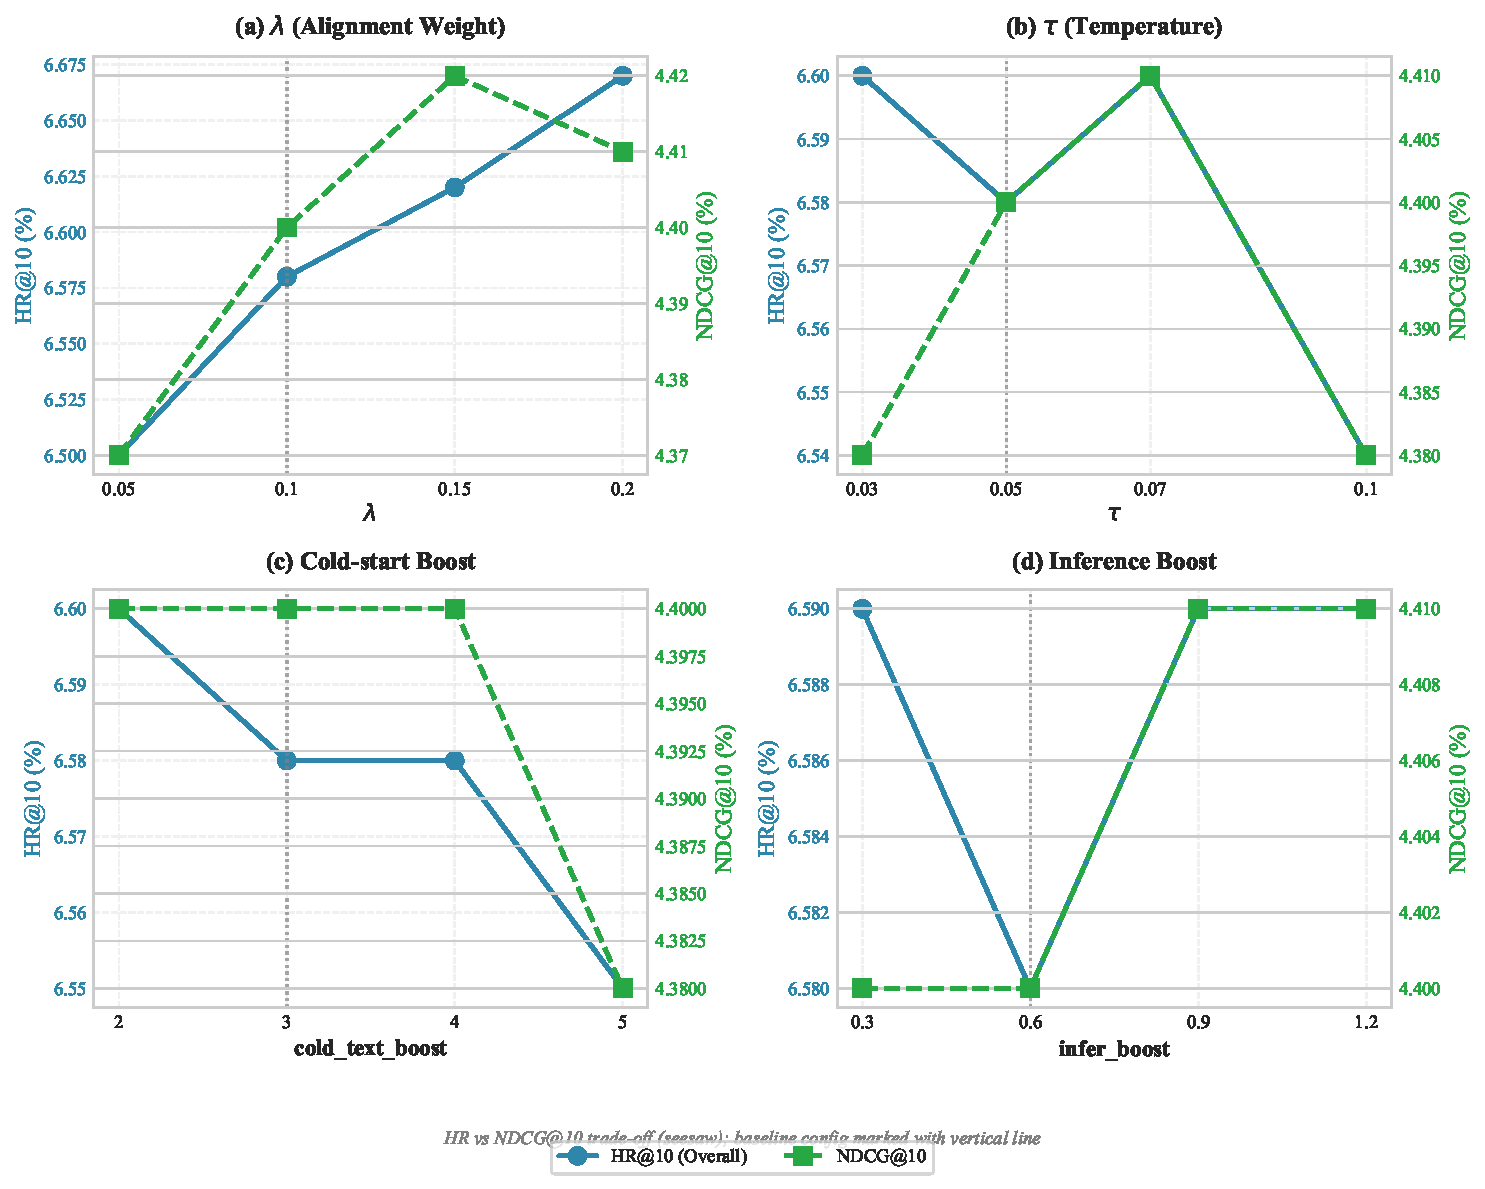
\includegraphics[width=\linewidth]{figures/sensitivity_tradeoff_ndcg.pdf}%
}{%
  \fbox{\parbox[c][0.25\textheight][c]{0.95\linewidth}{\centering
  \textbf{敏感性分析}\\
  运行 \texttt{plot\_sensitivity.py}}}%
}
\caption{Toys\&Games（7B）上的超参敏感性。各子图每次改变一个参数，其余保持默认值（竖虚线）。HR@10（实线，左轴）与 NDCG@10（虚线，右轴）在这些设置下稳定，HR@10 总变化低于 0.2 个百分点，NDCG@10 低于 0.05 个百分点。}
\label{fig:sensitivity}
\end{figure}

图~\ref{fig:sensitivity} 展示 \model 对 $\lambda$、$\tau$、$\beta$（式~\eqref{eq:cold_reweight}）与 $\beta_{\text{infer}}$（式~\eqref{eq:infer_boost}）在 Toys\&Games（7B）上的敏感性，每次变动一个参数，其余为默认值（$\lambda{=}0.10$，$\tau{=}0.05$，$\beta{=}3.0$，$\beta_{\text{infer}}{=}0.6$）。

\paragraph{对齐权重 $\lambda$ 与温度 $\tau$。}
两个对比超参均呈现平滑单峰曲线。HR@10 在 6.50\%（$\lambda{=}0.05$）到 6.67\%（$\lambda{=}0.20$）之间，跨度仅 0.17 个百分点；NDCG@10 在 $\lambda{=}0.15$ 达峰（4.42\%），网格内变化在 0.05 个百分点内。温度 $\tau$ 同样稳定：测试范围内 HR@10 变化 0.06 个百分点，NDCG@10 变化 0.03 个百分点（$0.03$--$0.10$）。表明对比目标对适度调参具有鲁棒性。

\paragraph{冷启动增强与推理增强。}
训练系数 $\beta$（式~\eqref{eq:cold_reweight}）对整体指标影响很小（HR@10 在 0.05 个百分点内，NDCG@10 在 0.02 个百分点内），因其主要影响训练期对低流行度物品的重加权。推理系数 $\beta_{\text{infer}}$ 对整体性能同样稳定（HR@10 在 0.01 个百分点内）。与式~\eqref{eq:infer_boost} 一致，它在推理时调节低流行度物品的文本依赖；在所测网格上整体 HR@10 与 NDCG@10 仍落在上述窄带内。

\paragraph{结论。}
这些超参对整体指标敏感性低，HR@10 总变化低于 0.2 个百分点，NDCG@10 低于 0.05 个百分点。使 \model 在实践中易于调参：默认配置已接近最优，从业者可调节 $\lambda$ 或 $\beta_{\text{infer}}$ 在整体与冷启动表现间权衡，而不易出现大幅回退。

\section{结论}
我们提出 \model，将显式交叉网络与多视角 \llm 文本对齐引入序列推荐。
Amazon Beauty 与 Toys\&Games 上的全量排序实验给出三条可操作建议：

\textbf{(1) TF-IDF 是出人意料的强基线。}
单独 \tfidf 相对仅 ID 已有可观增益（Beauty/Toys 上 HR@10 +2.6\%/+6.3\%），在投入 \llm 嵌入前应作为\textbf{首选}文本增强。

\textbf{(2) 相同带宽下多视角改善冷启动排序。}
在相同嵌入带宽（$4{\times}64$ 对 $1{\times}256$）下，多视角 \llm 提示取得最优冷启动排序质量：\model 在两数据集上 NDCG\_new@10 与 MRR\_new@10 最高，同时 Beauty 上缩小 HR\_new 与仅 ID 的差距（1.76\% 对 1.88\%），Toys 上超过仅 ID（2.04\% 对 1.92\%）。

\textbf{(3) 交叉网络决定 HR--MRR/NDCG 权衡。}
启用交叉以召回（HR）为代价提升排序质量（MRR/NDCG）；关闭则相反。直接对应部署：候选生成阶段关闭交叉，最终重排阶段启用交叉。

\smallskip\noindent
全部代码与配置文件见 \texttt{\url{https://anonymous.4open.science/r/recbole-multiview-D83A}}。

\bibliographystyle{unsrt}
\bibliography{refs}

%% 附录已按 RecSys 主会长文（8 页 + 参考文献）要求移除。
%% 辅助分析见匿名仓库：https://anonymous.4open.science/r/recbole-multiview-D83A

\end{document}
